\section{Evaluation}

\comment{

Giza provides fault tolerance through erasure coding across wide area networks while providing linearizability for its read and write operations. As such, there are currently no system that is specifically designed to serve as an alternative to Giza. However, we benchmark Giza’s performance against Cassandra and CockroachDB to illustrate the following points:

- In the common case, Giza’s Fast Paxos implementation of the metadata phase allows for lower latency writes for Giza when compared to Cassandra.

- While one could implement Giza’s metadata phase and data phase as a single distributed transaction, we illustrate through CockroachDB that doing so will degrade performance significantly.

In addition, we provide evaluation results for encoding scheme ranging from 2-1 in 3 data centers to 18-4 in 22 data centers to illustrate the flexibility of Giza as a front end.

}

For evaluation, we deploy Giza on top of the Microsoft Azure platform across up to 11 data centers (7 in North America, 2 in Europe and 2 in Asia). For each data center, we deploy a virtual machine that runs as the Giza node. As describe in section~\ref{sec:design}, all the Giza nodes are stateless. Upon receiving {\em get} or {\em put} requests, the Giza nodes execute the data and the metadata paths to read or write data objects.

%In each data center, we create a single virtual machines as a Giza node. We also create a number of Azure storage accounts. These storage accounts are local to individual DCs and allow access to Azure Blob storage and Azure Table storage in the DCs.

%We form \name storage account as a collection of the local Azure storage accounts. We also specify the erasure coding scheme for each account. For example, a North American only Giza storage account may apply $2+1$ erasure coding and consist of 4 data centers in the US, as xxx, xxx, xxx and xxx. A global Giza storage account may apply same coding and consist of 4 data centers across 3 continents, as xxx, xxx, xxx and xxx.

%As described in section~\ref{sec:design}, all the Giza nodes are stateless. Upon receiving {\em get} or {\em put} requests, the Giza nodes execute the data and the metadata paths to read or write data objects.

\begin{figure}
\begin{tabular}{c|c|c|c}
          & Coding & Data and Metadata DCs & Ping (max)\\
\hline
%US-2-1 	  & 2 + 1 & 3 & Central, South Central, West & Central, South Central, West & 46 ms \\
%US-6-1 	  & 6 + 1 & 7 & Central, South Central, West & Central, South Central, West & 71 ms\\ 
%jWorld-2-1 & 2 + 1 & 3 & Central, Europe North, Japan East & Central, Europe North, Japan East & 240ms\\
%World-6-1 & 6 + 1 & 7 & Central, South Central, West & Central, Europe North, Japan East & 241 ms\\
US-2-1 	  & 2 + 1 & US(3/3)                   & 46 ms \\
US-6-1 	  & 6 + 1 & US(7/3)                   & 71 ms\\ 
World-2-1 & 2 + 1 & US(1/1), EU(1/1), JP(1/1) & 240ms\\
World-6-1 & 6 + 1 & US(3/1), EU(3/1), JP(1/1) & 241 ms\\
\end{tabular}
\caption{Giza Configuration ( US(7/3) represents 7 data DCs and 3 metadata DCs in the US. )} 
\label{fig:dcconfig} 
\end{figure}

\subsection{Experimental Setup}
%For evaluation, we deploy Giza on top of the Microsoft Azure platform across up to 11 data centers (7 in North America, 2 in Europe and 2 in Asia). %As described in section~\ref{sec:design}, all the Giza nodes are stateless. Upon receiving {\em get} or {\em put} requests, the Giza nodes execute the data and the metadata paths to read or write data objects.
We run experiments using four configurations: 2-1-US, 2-1-World, 6-1-US and 6-1-World. Figure~\ref{fig:dcconfig} describes the data centers participating in each configuration, and the max ping latency between the DCs. 
Giza nodes are Azure virtual machines with 16 cores, 56 GB of RAM, and gigabit ethernet. For each Giza account, a locally redundant Azure Blob and Table storage account is created in every DC.

We also compare Giza with CockroachDB~\cite{cockroachdb}, an open source implementation of Google spanner. Our CockroachDB experiments use the 2-1-US configuration. In every data center, we run three CockroachDB instances, each writing to a dedicated HDD with no memory caching. We have configured the CockroachDB instances following the recommended production setting by the CockroachDB developers. For example, following the recommendation, we run NTP to synchronize clocks of different CockroachDB instances.

%We evaluate the latency performance of Giza and CockroachDB by running 1000 operations (for put and get) during the same timeframe. This is because the latency results obtained at different time throughout the day or week can vary significantly. 
 
%For all latency results, we report the 50th percentile. We refrain from using the 95th percentile due to the high variability of the tail distribution observed in public cloud platforms. Since the performance of Giza is determined by the performance of the underlying infrastructures (Azure Table and Azure Storage), we also  provide latency benchmark for Azure’s Table and Blob storages in Figure 5. Figure 5a shows the vm to local azure table latency for all the vms participating in the metadata path. The put and get latency are pretty consistent across vm with the put latency being around 60ms and the get latency being around 10ms. Figure 5b shows the vm to local azure storage latency. Here, the latency varies widely from vm to vm with some latencies being double of others. The storage latencies also increase with the object sizes.

%Our experiments involve a varying number of DCs in different configurations. In
%each DC, we deploy a single Azure virtual machine (16 cores, 56 GB of RAM, and
%gigabit ethernet) and create a storage account for accessing Azure blob and
%table storage. Both the blob and table storage are configured with the
%``locally redundant'' replication level.  Each \name node accesses the local
%DC's cloud storage and also proxies the storage requests from \name nodes in
%other DCs.  

%For CockroachDB experiments, we run a CockroachDB cluster spanning across
%multiple DCs.  We use the same set of Azure virtual machines and run a single
%CockroachDB node per DC. Our configuration of CockroachDB follows the
%recommended production settings by the developers of CockroachDB. For example,
%we run NTP to synchronize the clocks of different CockroachDB nodes. 

%We generate experimental workloads using the YCSB benchmark. In the generated
%workload, the probability of accessing a given key follows a Zipf distribution.
%We experiment with different object sizes ranging from 128KB to 4MB. 

%We experiment with four diffferent DC configurations, as shown in
%Figure~\ref{fig:dcconfig}.  These configurations correspond to different coding
%rates and different choices of DCs, either within US-only or spread across the
%world. The wide-area latency across different DCs plays an important role in 
%the performance of \name.  Figure~\ref{fig:dcconfig} reports the majority
%latency (measured as the latency required to get a response from a majority
%quorum of DCs) and the maximum latency between DCs.



\subsection{Metadata Path Optimization}
When comparing the performance between implementing the metadata path with Fast Paxos and Classic Paxos, we found two factors that are important in determining which configuration outperforms the other.  The first factor is whether the vm to local azure write latency is dominant in the metadata path and the second factor is the difference in the maximal distance between data centers in a fast quorum and a classic quorum. 

The performance of the metadata path is determined by the request latency between the coordinator and the table storage of the furthest data center in the quorum. Each request to a remote table storage is broken down into two parts: vm to vm latency and vm to local azure storage latency. From our previous analysis, the write latency from a vm to its local azure storage is around 60 milliseconds. The vm to vm latency is determined by the location of the data centers and can range from 20 milliseconds (us central to us south central) to 240 milliseconds (east Japan to north Europe). Figure~\ref{fig:metadata} illustrates the latency difference between the two Paxos schemes. The metadata path latency is broken down into three parts: query version latency, the table access latency, and the transfer latency. The query version latency, a simple read from the proposer’s local table to determine the possible highest version, is not part of the consensus protocol and is the same for both Fast and Classic Paxos. The table access latency is the local table access latency of the vm that is furthest away from the coordinator in the quorum. Since Classical Paxos requires two rounds and hence two table accesses, the Classic Paxos table access latency is consistently around twice the latency of the Fast Paxos table access. The transfer latency is the amount of time spent on network communication between the coordinator and the furthest vm in the quorum. Here the latency of the Classic Paxos, which incurs two round trip, is not strictly twice as much as the latency of the Fast Paxos. This is because the Classic quorum size is smaller than the Fast quorum size.

In the top row of figure, we see that when the vm to local azure storage latency dominates the metadata latency (in the case of the 2-1 US configuration), the latency of Fast Paxos metadata path is lower than that of the Classic Paxos metadata path no matter which region you start the request from. In addition, if the max distance between the data centers in a fast quorum is close to that in a classic quorum, the latency of the Fast Paxos metadata path is half of that of the Classic Paxos metadata path. In certain scenarios, it is possible for Classic Paxos to achieve lower latency than Fast Paxos. While we didn’t observe this in our two configurations, we see that if we start the request from North Europe in the 2-1 world configuration, the latencies are almost the same. This is because a Fast Paxos round requires a bigger quorum response and in this case, a fast quorum consists of North Europe, US, and East Japan. The vm to vm latency between North Europe and East Japan is 240 milliseconds while the vm to vm latency between North Europe and US is only 102 milliseconds. Hence the max distance between data centers in the classic quorum (US and North Europe) is less than half of that of the fast quorum. The scenario in which the Classic Paxos scheme outperforms the Fast Paxos scheme is:
\[max\_dist(F) > 2 * max\_dist(Q) + \textrm{extra table access}
\]
where F is the fast quorum size and Q is the classic quorum size.
%\begin{figure*}[t]
%%  \centerline {
%      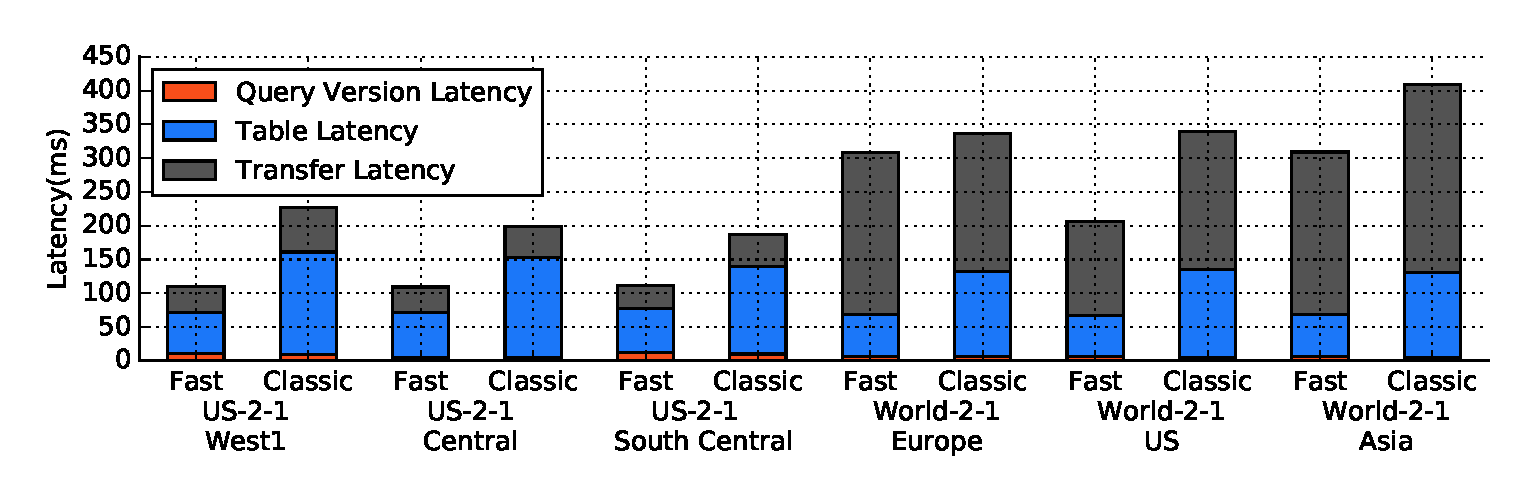
\includegraphics[width=0.75\linewidth]{plots/metadata}
%      \caption{Fast Paxos and Classic Paxos Comparison}
%      \label{fig:metadata}
%%  }
%\end{figure*}


\begin{figure*}
\centering
\begin{minipage}{.7\textwidth}
  \centering
  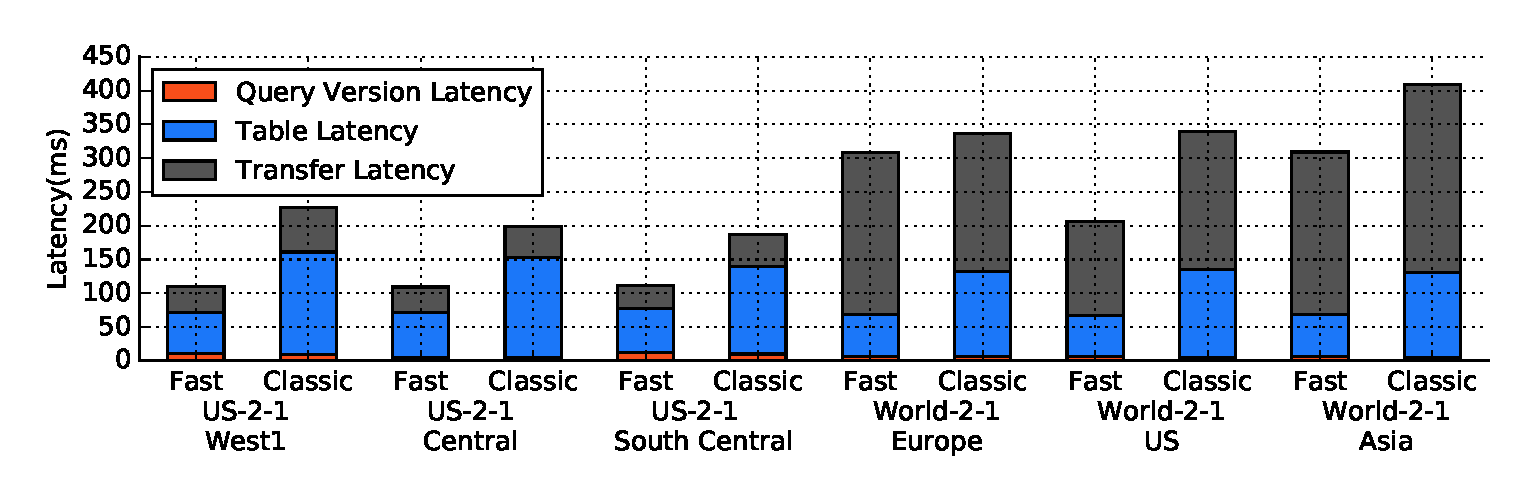
\includegraphics[width=\linewidth]{plots/metadata}
  \caption{Fast Paxos and Classic Paxos Comparison}
  \label{fig:metadata}
\end{minipage}%
\begin{minipage}{.3\textwidth}
  \centering
      \includegraphics[width=\textwidth]{plots/contention_bar}
      \caption{Contention vs No Contention}
      \label{fig:gizacontentionbar}
\end{minipage}
\end{figure*}


\subsection{\name Latency}
The design of Giza went through multiple iterations and this section illustrates the performance gain in latency for each iteration. In our workloads, the predominant object size is 4MB. Hence, we focus on the {\em put} and {\em get} latency of 4MB objects in the evaluation. For the interest of space, we chose the 2-1-World configuration where US Central generates all requests as representative of the performance gain seen in other configurations.

\subsubsection{Giza Put Latency}
%\subsubsection{Giza Latency}

%\begin{figure}[t]
%  \centerline {
%    \begin{subfigure}{0.20\textwidth}
%      \includegraphics[width=\linewidth]{plots/giza_lat_put}
%      \caption{Put}
%      \label{fig:eval_giza_put}
%    \end{subfigure}
%    \begin{subfigure}{0.20\textwidth}
%      \includegraphics[width=\linewidth]{plots/giza_lat_get}
%      \caption{Get}
%      \label{fig:eval_giza_get}
%    \end{subfigure}
%  }
%  \caption{\name Overall Latency}
%  \label{fig:geo_tpcc}
%\end{figure}

%%% Local Variables:
%%% mode: latex
%%% TeX-master: "main"
%%% End:


Figure~\ref{fig:eval_giza_put} shows the \name overall {\em put} latency for 4MB data. We compare Giza with two previous iterations where the metadata path is not parallelized with the data path. In the first iteration, Giza runs the data path first. Upon success, Giza runs the metadata path with Classic Paxos implementation. In the second iteration, we replaced Classic Paxos with Fast Paxos and see the performance gain described previously. While parallelizing metadata path with data path can results in extra metadata or data clean up if one of them fails, the performance gain is significant. We also included a baseline which is the blob store latency from the requester (US Central) to the furthest data center (Japan East).

The results show that \name's performance beats the other two alternatives in the common case and has closest
latency to the baseline. The median latency of \name put is 374 ms, which is only 30 ms
higher than the baseline. This is due to the latency of erasure coding 4mb data. On the other hand, the serial classic paxos version takes 
xxx ms, and the serial fast paxos version takes xxx ms.

\subsubsection{Giza Get Latency}

Similar to the put test, we did a \name get test, as shown in Figure~\ref{fig:eval_giza_get}. The alternative design here is the non-optimistic {\em get } where the most current version for a blob is not assumed to be stored in the current data center. Hence, the metadata path and data path are executed sequentially. We see the performance gain from the pessimistic version with a median latency xxx ms to the optimistic version's xxx ms. Giza's get latency is higher than the baseline by xxx ms. The gap between \name and baseline is higher because in the get operation \name needs to do a local table retrieve first before starting the datapath. 

%The results are expected. The \name put latency consists of a 
%metadata put latency and datapath latency. 



\comment{

% \begin{figure}[!h]
% \centering
%   \subfloat[Giza Put 99th Percentile]{\includegraphics[width=0.5\textwidth]{images/write_latency}\label{fig:f1}}
%   \subfloat[Giza Get 99th Percentile]{\includegraphics[width=0.5\textwidth]{images/write_latency}\label{fig:f2}}
% \caption{Comparison of latency of the four configurations}
% \end{figure}
\subsection {Different Configurations}
\sm {
  In this section, I will provide a latency graph (put and get) of all the 4 different configurations. The x axis is the size of the objects and the y axis is the latency. This section is to illustrate the trade off between storage efficiency and read latency. 
}

}

\subsection{Footprint Impact}


\begin{figure}[t]
%  \centerline {
    \begin{subfigure}{0.40\textwidth}
      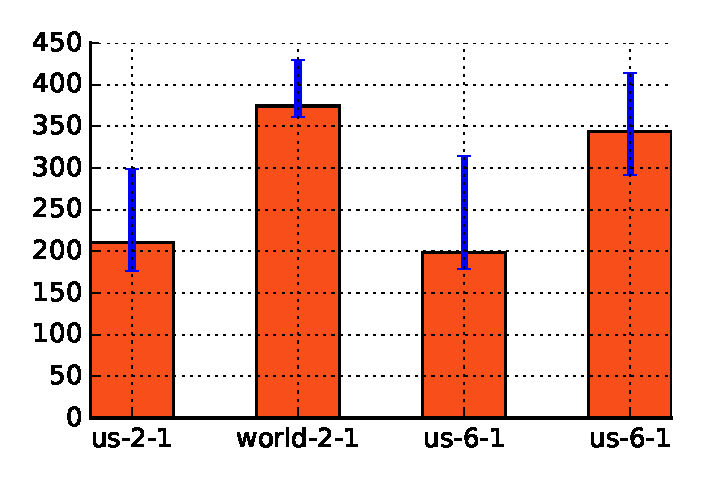
\includegraphics[width=\linewidth]{plots/giza_four_put}

      % \placeholder{
      %   x-axis: \# clients / partition\\
      %   y-axis: cluster throughput\\
      %   lines: \name{}, OCC, 2PL, TAPIR\\
      %   }
%                \vspace{-1\baselineskip}
      \caption{Put}
      \label{fig:eval_giza_put_four}
    \end{subfigure}
%    \begin{subfigure}{0.33\textwidth}
%      \includegraphics[width=\linewidth]{figs/graphs/multi_dc/tpcc/tpcc_NEW_ORDER_tpcc_client_lat90.eps}
%
%      % \placeholder{
%      %   x-axis: \# clients / partition\\
%      %   y-axis: latency (median, p90, p99)\\
%      %   (maybe only show median and p99 or just median and report typical distribution)\\
%      %   lines: \name{}, OCC, 2PL, TAPIR\\
%      % }
%      \caption{90\% Latency}
%      \label{fig:geo_tpcc_latency}
%    \end{subfigure}
    \begin{subfigure}{0.40\textwidth}
      \includegraphics[width=\linewidth]{plots/giza_four_get}

      % \placeholder{
      %   x-axis: \# clients / partition\\
      %   y-axis: commit rate\\
      %   lines: \name{}, OCC, 2PL, TAPIR\\
      % }
      %\includegraphics[width=\linewidth]{fig/kodiak/tpcc_mix_10_nlog_ct_cr.pdf}
%                \vspace{-1\baselineskip}
      \caption{Get}
      \label{fig:eval_giza_get_four}
    \end{subfigure}
%  }
  \caption{Performance for \name in different setups}
\end{figure}

%%% Local Variables:
%%% mode: latex
%%% TeX-master: "main"
%%% End:


\name offers customers the flexibility to choose the set of data centers, as well as the erasure coding schemes. As the main goal of Giza is storage cost reduction, we want to encourage erasure encoding with more numbers of data fragments. Because Giza’s latency performance is determined by the max of the data path and the metadata path and data path is most often the dominant latency, erasure coding with higher number of data fragments can actually improve latency performance. This is because more data fragments means that less bytes are sent to each storage, reducing the overall data path latency. Figure~\ref{fig:eval_giza_put_four} and  Figure~\ref{fig:eval_giza_get_four} illustrate this in our four configurations with 4MB data, with all requests generated from US-Central. This improvement of performance with higher configurations occurs when the max distance between the data centers in the higher configuration group (7 data centers) is not more than the max distance between the data centers in the lower configuration group (3 data centers).


\subsection{Comparing Giza with CockroachDB}
We only compare Giza's US-2-1 configuration with CockroachDB since CockroachDB currently does not fully support world wide geo-replication. We also don't include comparison to  the US-6-1 scheme in the interest of space.

We implemented Giza put and get as transactions. Because CockroachDB fully supports ACID transactions, we can use CockroachDB to build a strongly consistent key value store that encodes objects across multiple data centers. To do this, we create four different tables: a metadata table and 3 tables that serves as key value stores for each of the data centers. The metadata table is replicated across all three data centers, once in each data center, and can tolerate one data center failure. Each of the remaining tables is replicated 3 times in its respective data center. Since CockroachDB uses Paxos for replication, the write critical path only requires the completion of 2 our of 3 replications. This is to match the local replication factor in the Azure storage where each blob is synchronously replicated once on the write critical path.

The implementation of Giza put as a transaction consists of storing each data fragments at the corresponding key value table and storing the metadata information in the metadata table. This transaction involves all four tables for a 2,1 configuration. Figure~\ref{fig:eval_cock_put} compares the latency performance of the two. Here Giza outperforms CockroachDB significantly.
However CockroachDB is currently not suited for storing large objects, as specified by the developers. We also tested CockroachDB with 128KB objects (This is 64KB after encoding, which is the largest size CockroachDB can handle before large performance degradation). As seen in Figure~\ref{fig:eval_cock_put2}, even with just 128KB, the performance of CockroachDB is still worse than the performance of Giza even with 4MB objects.

The implmentation of Giza get as a transaction consists of reading from the metadata table and reading the minimum amount of data fragments, in this case two, from the key value tables. This transaction involves three out of the four tables. Figure~\ref{fig:eval_cock_get} shows the performance comparison. Here CockroachDB performs better than Giza. However, this is not surprising. CockroachDB reads directly from hdd, which is faster than Giza's read from the Azure storage.


%To set up CockroachDB, we use the same azure virtual machine instances and run a single CockroachDB node. We followed the recommended production settings by the developers of CockroachDB when deploying these instances. For example, on the same virtual machine, we also run NTP to provide moderately accurate time to preserve data consistency. Other optimizations can be found on the CockroachDB website. We only benchmark CockraochDB against Giza in the 3 dc cluster scenario since we want the fault tolerance level to be the same for the comparisons.
%Since variability in latency is a factor when benchmarking cloud storage, we run all our experiments at approximately the same time.
%Since latency is an issue, we run all our experiments at around the same time.
%We experimented with different erasure coding schemes
% For all experiments, we deployed a single virtual machine (16 cores, 56 GB of RAM, 800 GB SSD, and gigabit ethernet) for each geographical region. We use the same virtual machines for setting up the Cassandra and CockroachDB clusters. The client issuing the requests runs on one of the virtual machine that is also part of the cluster. 
% To set up Giza, we also had to deployed both a table service and a blob service provided by the cloud service platform. The granularity of replication for these services varies from provider to provider but we always choose the replication level to match that of the regional replication. This means that as long as there’s no dc outage, the data would not be lost. For each data center, we run a Giza node frontend with the virtual machine. The Giza node can service requests from a client running in the virtual machine. In addition, requests to its local table and blob storage from other Giza nodes also go through the Giza node frontend in the form of an RPC call. This is to avoid unecessary WAN round trips when dealing with complicated table and blob storage operations. 

\begin{figure}[t]
%  \centerline {
      \includegraphics[width=\linewidth]{images/cockroach_vs_giza_put}
      \caption{CockroachDB vs Giza with various object sizes}
      \label{fig:eval_cock_put}
%  }
\end{figure}

\begin{figure}[t]
%  \centerline {
      \includegraphics[width=\linewidth]{images/cockroach_vs_giza_put_128}
      \caption{CockroachDB vs Giza with various object sizes}
      \label{fig:eval_cock_put2}
%  }
\end{figure}

\begin{figure}[t]
%  \centerline {
      \includegraphics[width=\linewidth]{images/cockroach_vs_giza_get}
      \caption{CockroachDB vs Giza with various object sizes}
      \label{fig:eval_cock_get}
%  }
\end{figure}
%%% Local Variables:
%%% mode: latex
%%% TeX-master: "main"
%%% End:


%\sm {
%  In this section, I will have two graphs. One comparing Giza's full write path with CockroachDB's full replication. Another one is comparing the metadata path with cockroach db. This is to show, hopefully, that the fast paxos scheme is better. I will probably have 3 graphs each making request from one of the three datacenters. Due to multipaxos, there might be extra latency for cockroachdb's case.
%}
%We benchmark the performance of Giza with CockroachDB in two cases. In the first case, we use CockroachDB as a geo-replicating blah blah blah. Here is the result.
%In the second case, we used cockroachdb's transaction to simulate what we are doing with Giza. Blah blah blah, here is the result.
%64K $\sim$ 16MB

%X-axis: Value size
%Y-axis: 50\% Read latency

%X-axis: Value size
%Y-axis: 90\% Read latency

%X-axis: Value size
%Y-axis: 99\% Read latency

%Same for write

%[adding cpu results in a table]

% \subsection{Large object}
% 256MB $\sim$ 1GB

% X-axis: Value size
% Y-axis: Average Read latency

% X-axis: Value size
% Y-axis: Average Write latency


% \subsection{Contention}

% Fixed object size
% X-axis: zipf coefficient
% Y-axis: 50\%, 90\%, 99\% Read/Write Latency


% \subsection{Real workload}
% Table.


%%% Local Variables:
%%% mode: latex
%%% TeX-master: "main"
%%% End:

